\documentclass[letterpaper,twocolumn,10pt]{article}
\usepackage{usenix2019_v3}

% to be able to draw some self-contained figs
\usepackage{tikz}
\usetikzlibrary{positioning,calc,decorations}
\usepackage{enumitem} % For more control over list formatting
\usepackage{calc}     % For calculating widths if needed
\usepackage{amsmath}

% inlined bib file
\usepackage{filecontents}

%-------------------------------------------------------------------------------
\begin{filecontents}{\jobname.bib}
%-------------------------------------------------------------------------------
@Book{arpachiDusseau18:osbook,
  author =       {Arpaci-Dusseau, Remzi H. and Arpaci-Dusseau Andrea C.},
  title =        {Operating Systems: Three Easy Pieces},
  publisher =    {Arpaci-Dusseau Books, LLC},
  year =         2015,
  edition =      {1.00},
  note =         {\url{http://pages.cs.wisc.edu/~remzi/OSTEP/}}
}
@InProceedings{waldspurger02,
  author =       {Waldspurger, Carl A.},
  title =        {Memory resource management in {VMware ESX} server},
  booktitle =    {USENIX Symposium on Operating System Design and
                  Implementation (OSDI)},
  year =         2002,
  pages =        {181--194},
  note =         {\url{https://www.usenix.org/legacy/event/osdi02/tech/waldspurger/waldspurger.pdf}}}
\end{filecontents}

%-------------------------------------------------------------------------------
\begin{document}
%-------------------------------------------------------------------------------

%don't want date printed
\date{}

% make title bold and 14 pt font (Latex default is non-bold, 16 pt)
\title{\Large \bf Secure IVSHMEM Protocol}

%for single author (just remove % characters)
\author{
{\rm Your N.\ Here}\\
Your Institution
\and
{\rm Second Name}\\
Second Institution
% copy the following lines to add more authors
% \and
% {\rm Name}\\
%Name Institution
} % end author

\maketitle




%----------Figure: Channel Separation-----------------
\begin{figure*}[ht]
\begin{center}
  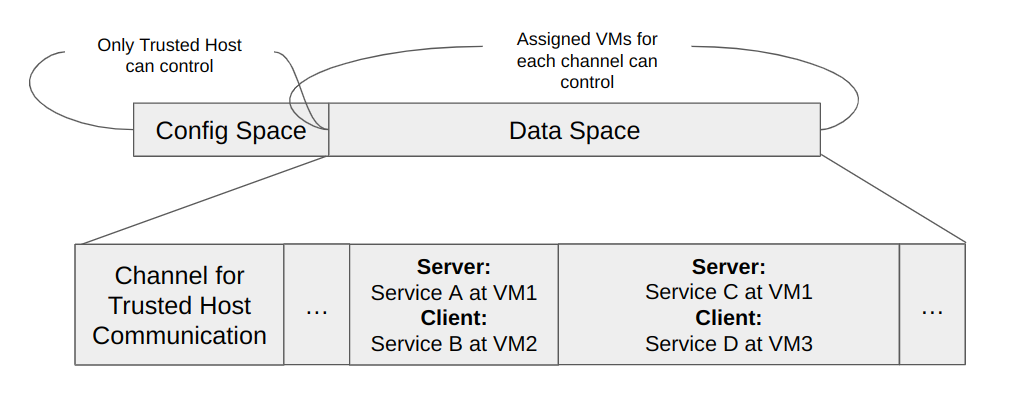
\includegraphics[width=\textwidth]{./figures/channel_separation.png}
\end{center}
\caption{\label{fig:channel_separation} channel separation figure 
  caption's text. }
\end{figure*}
%% %---------------------------

%-------------------------------------------------------------------------------
\begin{abstract}
%-------------------------------------------------------------------------------
Your abstract text goes here. Just a few facts. Whet our appetites.
Not more than 200 words, if possible, and preferably closer to 150.
\end{abstract}


%-------------------------------------------------------------------------------
\section{Introduction}
%-------------------------------------------------------------------------------

The automotive industry is rapidly evolving, driven by advances in semiconductor technology that have shifted system architectures from traditional microcontrollers (MCUs) to powerful Systems-on-Chip (SoCs). This evolution not only enhances computational capabilities but also paves the way for Software-Defined Vehicles (SDVs), where flexibility, scalability, and rapid updates are paramount. In SDVs, virtualization technology plays a crucial role by enabling the coexistence of multiple virtual machines (VMs) on a single hardware platform, ensuring isolated yet efficient execution of diverse applications. For example, modern cockpit domain controllers often deploy separate VMs for real-time operations (RTOS) and infotainment systems, which is essential for balancing performance and safety.

Inter-VM communication in these environments is critical. Traditional approaches, such as TCP/UDP over a network stack or even UART-based messaging, often fall short in terms of speed and resource efficiency. Alternative solutions like VirtIO offer a para-virtualized communication mechanism through ring buffers (VirtQueues), but they do not fully leverage the benefits of shared physical memory. IVSHMEM (Inter-VM Shared Memory) addresses these limitations by mapping each VM's virtualized PCI device to a common physical memory region, allowing rapid data exchange through shared memory. Despite its performance advantages, this method introduces significant security challenges; multiple VMs accessing the same memory space creates vulnerabilities where a compromised or malicious VM could potentially access or modify data belonging to another VM.

This concern is particularly acute in scenarios where critical systems interact with less secure environments. For instance, when an RTOS communicates with an Android-based infotainment VM, there is a tangible risk that a malicious application within Android might tamper with the shared memory region. Such tampering could result in attacks ranging from man-in-the-middle to eavesdropping, ultimately compromising system stability and safety.

In response to these challenges, we propose a secure protocol designed specifically for IVSHMEM communication in automotive systems. Our approach introduces robust security measures on top of the IVSHMEM framework, ensuring data integrity and access control even in an environment with inherent vulnerabilities. While our protocol does introduce some performance overhead, we have implemented novel techniques to mitigate this impact, ensuring that the overhead remains minimal relative to the performance gains achieved by shared memory communication.

In this paper, we provide a detailed analysis of the security threats associated with IVSHMEM, explore the limitations of existing inter-VM communication methods, and describe our protocol's architecture and mitigation strategies. Through comprehensive evaluation, we demonstrate that our secure protocol successfully balances the need for robust security with the high-performance requirements of modern automotive systems and SDVs.

\section{Background}

We explore the evolution of shared memory IPC—from its origins in minimizing data copying in single OS environments to its advanced application in inter-VM communication—and examine the challenges of establishing secure channels over inherently insecure mediums.

\subsection{Shared Memory Inter-Process Communication (IPC)}

Shared memory IPC is a communication mechanism that allows multiple processes running on the same operating system to access a common memory region. This method was originally introduced to avoid redundant data copies between processes, thereby enhancing performance. The concept has been extended to inter-VM communication, where co-located virtual machines (VMs) on the same host exchange data via a shared memory channel. Instead of routing data through the host operating system or hypervisor—an approach that incurs additional overhead—the sender VM writes data directly into a shared memory region and then notifies the receiver VM via an interrupt. This streamlined process significantly accelerates communication between VMs.


OpenMPI - Job Isolation?
Boost Interprocess?

\subsection{IVSHMEM: Mechanism and Architecture}


IVSHMEM (Inter-VM Shared Memory) is a specialized implementation of shared memory IPC designed for virtualized environments. It emulates a virtual PCI device to expose the shared memory's base address and size to guest VMs. The design leverages the standardized PCI configuration to facilitate memory mapping and efficient communication. Specifically, IVSHMEM utilizes:

- **BAR0 (Base Address Register 0):** This region (256 bytes of MMIO) holds the device registers, which control the operation of the virtual device.
- **BAR1:** It contains the MSI-X table and Pending Bit Array (PBA), primarily used by the IVSHMEM doorbell mechanism for signaling interrupts.
- **BAR2:** This is mapped to the shared memory object, providing a direct communication channel between VMs.

The doorbell interrupt mechanism enabled by this configuration allows VMs to notify one another when new data is available, ensuring efficient core utilization and reducing latency in inter-VM communication.

%----------Figure: handshake -----------------
\begin{figure}[ht]
\begin{center}
  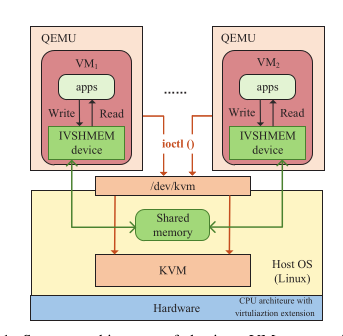
\includegraphics[width=0.95\linewidth]{./figures/ivshmem_arch.png}
\end{center}
\caption{\label{fig:ivshmem_arch} IVSHMEM architecture figure 
  caption's text. }
\end{figure}
%% %---------------------------




\subsection{Security Concerns of Shared Memory}
While shared memory IPC within a single operating system benefits from well-established security mechanisms—such as file access controls, sandboxing, and enhanced security modules like SELinux or AppArmor—IVSHMEM presents unique challenges. In a traditional OS environment, the operating system enforces strict access controls over shared memory regions, ensuring that only authorized processes can read or write data. However, when multiple, potentially untrusted VMs share the same memory space, these protections are significantly diminished. A compromised or malicious VM could easily access or tamper with data in the shared region, leading to unauthorized data disclosure, corruption, or even system instability. This risk is compounded by the fact that the emulated PCI device, which exposes the shared memory, does not inherently enforce robust access control policies among the VMs.


\subsection{Secure Communication Over Insecure Channels}

The challenge of ensuring secure communication in IVSHMEM environments is analogous to securing communication over the Internet, where multiple parties exchange information over an inherently insecure channel. In the realm of network communications, protocols such as TLS rely on key exchange mechanisms, mutual authentication, and end-to-end encryption to safeguard data integrity and confidentiality. Similarly, secure multi-party communication techniques—such as Diffie-Hellman key exchange and advanced encryption standards—are employed to establish trust even when the channel is compromised.

In the context of IVSHMEM, the situation is even more complex because multiple services must share the same restricted memory space as a communication channel. This necessitates the design of a secure protocol that not only ensures confidentiality and integrity—akin to TLS or other network security protocols—but also accommodates the shared nature of the memory resource. Our research addresses these challenges by proposing a secure protocol that implements robust cryptographic techniques to protect the data transmitted via IVSHMEM, while also mitigating the performance overhead typically associated with such security measures.



Through this background, we highlight the evolution from traditional shared memory IPC to advanced inter-VM communication methods like IVSHMEM, outline its architectural underpinnings, and discuss the critical security concerns that arise when untrusted VMs share a common memory resource. This sets the stage for our proposed solution, which aims to secure inter-VM communication in automotive systems without compromising on the performance benefits of shared memory mechanisms.




\section{The need for Secure IVSHMEM Protocol}

blah

\subsection{Threat Model}


untrusted VMs
replay attacks
man in the middle attacks
eavesdropping



\subsection{General Purpose of Secure IVSHMEM Protocol}

blah blah blah

\subsection{Performance Mitigation}

blah blah blah



\section{Design Proposal (or) Secure IVSHMEM Protocol}

blah blah blah




\subsection{Service-based Channel Separation}

Our design divides the IVSHMEM architecture into two primary sections: the \textbf{Control Section} and \textbf{the Data Section}. The Control Section is a fixed-size region where a trusted host stores dynamic configurations related to data allocation, while the Data Section is where virtual machines (VMs) actually read and write data through their assigned channels. Importantly, only the trusted host has permission to modify data in the Control Section, and each VM is restricted to reading and writing only to its designated channels within the Data Section.


The \textbf{Data Section} comprises multiple channels, with each channel serving as a dedicated buffer space for a specific server and client service pair. For each pair, a dedicated channel is allocated, and the Control Section dynamically adjusts its size based on the activation of channels.

For example, consider a scenario where Service A in VM1 needs to send data to Service B in VM2. In this case, the trusted host allocates an initial channel with a buffer size of 16 KB. The control information for this allocation is written into the Control Section, and only Service A and Service B are permitted to access the channel’s buffer. Additionally, the size of the channel buffer can be adjusted (enlarged or shrunk) based on the usage patterns between the services.

An exception to this rule is the first channel in the Data Section. This channel is of a fixed size and is exclusively used for communication between the trusted host and the VMs—for instance, during the initial handshake when a VM sends data to the trusted host. All VMs have access to this channel.


The \textbf{Control Section} maintains metadata about buffer assignments and channel usage. Its structure includes shared variables and an array of channel structures, which are described below:

\begin{description}[leftmargin=0.5cm, labelindent=0cm]
  \item[\textbf{free\_start\_offset} (int):] 
    Points to the next available space for a new buffer allocation.
  \item[\textbf{num\_active\_channel} (int):] 
    Tracks the number of currently active channels.
  \item[\textbf{control\_lock} (lock):] 
    Ensures thread-safe modifications during resizing operations.
  \item[\textbf{channels} (array of channel structures):] 
    Holds metadata for each communication channel.
    \begin{description}[leftmargin=0.5cm]
      \item[\textbf{service\_id} (int):] 
        The service ID as notified by the hypervisor.
      \item[\textbf{client\_process\_id} (int):] 
        An identifier used for granular access control.
      \item[\textbf{server\_service\_id} (int):] 
        The identifier for the server-side service.
      \item[\textbf{server\_process\_id} (int):] 
        The process identifier for the server.
      \item[\textbf{data\_address} (pointer):] 
        The address of the assigned channel buffer.
      \item[\textbf{data\_size} (size):] 
        The size of the assigned channel buffer.
    \end{description}
\end{description}

Channels utilize the metadata provided in the Control Section to read from and write to the designated buffer regions.


\subsection{Granualr Access Control}


To enhance the security of the IVSHMEM framework, we propose a granular access control mechanism that restricts access to the shared memory channels on a per-application basis. This mechanism is implemented via a dedicated kernel module that operates on top of the IVSHMEM device driver.



\subsubsection{Kernel Module Integration}

The kernel module intercepts all read and write system calls directed at the IVSHMEM device. By doing so, it validates each access request against a predefined set of policies that specify which host or VM is permitted to interact with a given channel. Notably, the module consults the IVSHMEM control section to enforce these access control rules, ensuring that only the authorized party can access the corresponding channel buffer.



\subsubsection{Channel-Specific Enforcement}

Each channel within the Data Section is allocated to a specific pair of services (e.g., a server and a client). The kernel module uses the control section's metadata to determine channel assignments and enforces strict access control, permitting operations only on the designated channel buffers.



\subsubsection{Disabling Memory Mapping}

For security reasons, the use of `mmap` is explicitly prohibited for the IVSHMEM device. While this may sacrifice some of the performance benefits typically associated with memory mapping, it is a necessary trade-off to prevent unauthorized access and to maintain robust security across the system.

This granular access control approach not only reinforces data isolation among different VMs and the host but also mitigates potential risks associated with unauthorized memory access, ensuring that the system's security is prioritized over marginal performance gains.



\subsection{Hypervisor Mediated Handshake Protocol}

We examine why a secure handshake protocol is essential for IVSHMEM communication by identifying its potential security risks, demonstrate how our scenario differs from conventional communication protocols, and introduce our detailed proposed handshake design.






\subsubsection{The Need for Secure Handshake}


\textbf{Mitigating Spoofing/Impersonation Risks:}

Since the trusted host (e.g., dom0 in Xen, SOS in ACRN, or the host in QEMU/KVM) does not inherently know which service is associated with which endpoint, it must ensure that a malicious entity cannot impersonate a legitimate client or server. The protocol must defend against such spoofing attacks by validating the identity of each endpoint before establishing a dedicated channel.
    
\textbf{Securing Data in an Untrusted Environment:}

The IVSHMEM memory space, used for key exchange and initial communication, is inherently insecure and can be monitored by potentially untrusted VMs. Encrypting sensitive data—including credentials and key exchange parameters—ensures that any eavesdropped information remains unintelligible and useless to an attacker.
    
\textbf{Robust Key Exchange Over Insecure Channels:}

Although the key exchange takes place over an untrusted channel, the protocol employs strong cryptographic techniques (e.g., ephemeral Diffie-Hellman) to generate a shared secret. This secret is then used to secure all subsequent communications between the client and server, effectively mitigating the risks associated with the insecure IVSHMEM space.


The following handshake protocol leverages these principles to ensure that even in an environment where the initial contact is over an untrusted channel, the eventual communication between client and server is both authenticated and secure. This design effectively addresses the threat of impersonation or spoofing by mandating robust credential validation and encryption from the very first step of the handshake process.





\subsubsection{The Difference from Conventional Security Protocols}

This scenario is similar to other network communication contexts—such as secure exchanges over VPNs or encrypted Wi-Fi networks—in that multiple parties must communicate over an inherently insecure channel. In our proposal, mutual authentication is implemented much like mTLS, where both the client and server prove their identities, and service-level authentication is ensured similarly to EE2E, confirming that the specific service endpoints are legitimate. These mechanisms verify credentials and secure connections, aligning with established practices in conventional protocols.

However, our proposed protocol is different from the conventional internet based security protocol in that 1) The trusted host (hypervisor) is not merely a passive participant but is responsible for allocating finite resources and establishing the communication channel  and 2) The hypervisor functions as a certification authority (CA), validating service credentials and orchestrating the creation of dedicated secure channels between clients and servers. 

The detailed handshake protocol steps are provided below, demonstrating the secure bootstrapping and key negotiation processes that lead to the establishment of a confidential IVSHMEM channel.






\subsubsection{Protocol Steps}

%----------Figure: handshake -----------------
\begin{figure}[ht]
\begin{center}
  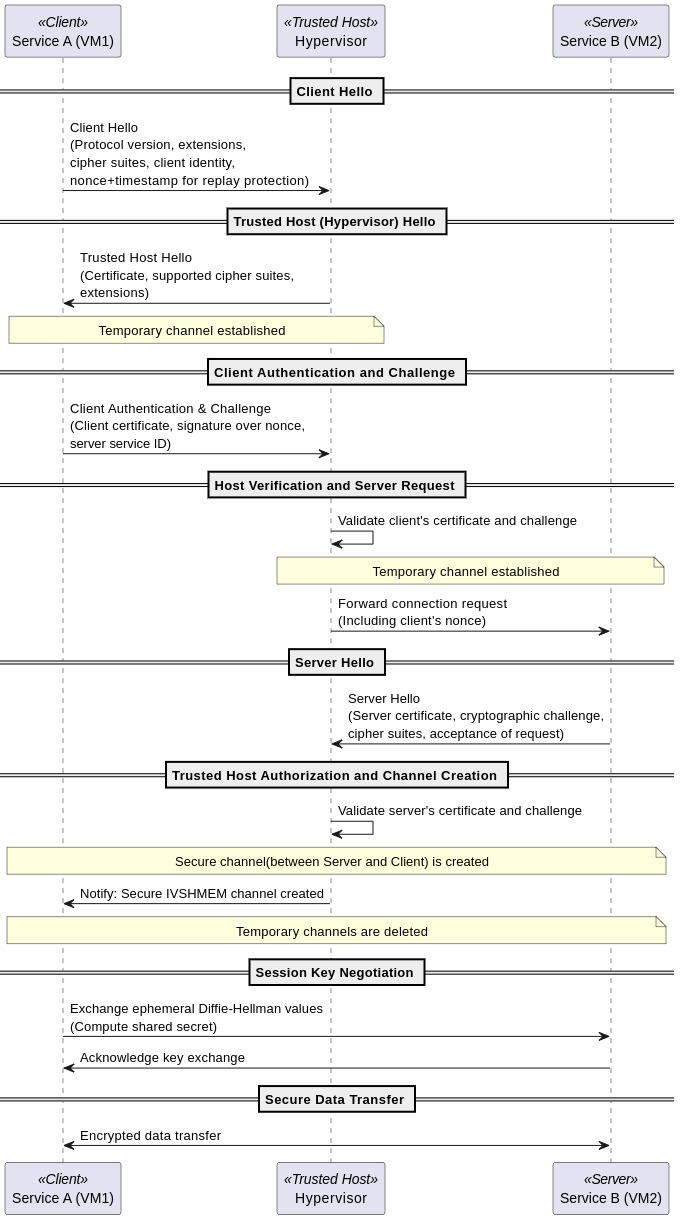
\includegraphics[width=0.95\linewidth]{./figures/ivshmem_handshake.png}
\end{center}
\caption{\label{fig:handshake} handshake figure 
  caption's text. }
\end{figure}
%% %---------------------------



% ----------- Handshake Protocol ------------
\begin{enumerate}[label=\arabic*.]
  \item \textbf{Client Hello:}
    \begin{itemize}
      \item \textbf{Purpose:} Initiate the handshake and propose communication parameters.
      \item \textbf{Message Contents:}
        \begin{itemize}
          \item Protocol version and supported extensions.
          \item A list of supported cipher suites.
          \item Client identity details (service ID, process ID, VM ID).
          \item A nonce combined with a timestamp or sequence number for replay protection.
        \end{itemize}
    \end{itemize}
    
  \item \textbf{Trusted Host (Hypervisor) Hello:}
    \begin{itemize}
      \item \textbf{Purpose:} Acknowledge the client's request and provide trusted credentials.
      \item \textbf{Message Contents:}
        \begin{itemize}
          \item The trusted host’s certificate.
          \item Supported cipher suites (if negotiation is to be assisted).
          \item Any additional protocol extensions.
        \end{itemize}
      \item \textbf{Action:} A temporary secure channel is created between the client and the trusted host.
    \end{itemize}

  \item \textbf{Client Authentication and Challenge:}
    \begin{itemize}
      \item \textbf{Purpose:} Enable explicit mutual authentication.
      \item \textbf{Message Contents:}
        \begin{itemize}
          \item The client’s certificate.
          \item A cryptographic challenge (e.g., a signature over a nonce) to prove possession of the corresponding private key.
          \item The intended server’s service ID.
        \end{itemize}
    \end{itemize}
    
  \item \textbf{Host Verification and Server Request:}
    \begin{itemize}
      \item \textbf{Purpose:} Verify the client's credentials and initiate communication with the server.
      \item \textbf{Action:}
        \begin{itemize}
          \item The trusted host validates the client’s certificate and challenge.
          \item Upon successful validation, the trusted host creates a temporary channel for the server and forwards a secure connection request to the server, including the nonce.
        \end{itemize}
    \end{itemize}
    
  \item \textbf{Server Hello:}
    \begin{itemize}
      \item \textbf{Purpose:} Server passes its credentials and decision to accept the client’s request.
      \item \textbf{Message Contents:}
        \begin{itemize}
          \item The server’s certificate.
          \item A server-side cryptographic challenge (to verify the server’s private key).
          \item Its supported cipher suites.
          \item Acceptance of the client’s request.
        \end{itemize}
    \end{itemize}
    
  \item \textbf{Trusted Host Authorization and Channel Creation:}
    \begin{itemize}
      \item \textbf{Purpose:} Establish a secure, dedicated IVSHMEM channel for data transfer between the server and client.
      \item \textbf{Action:}
        \begin{itemize}
          \item The trusted host verifies the server’s certificate and the corresponding challenge.
          \item The trusted host creates a communication channel for the server and client and notifies the client.
          \item The trusted host deletes temporary channels previously established with both the client and the server.
        \end{itemize}
    \end{itemize}
    
  \item \textbf{Session Key Negotiation:}
    \begin{itemize}
      \item \textbf{Purpose:} Finalize the authentication process and derive session keys.
      \item \textbf{Actions:} The client and server use the provided ephemeral Diffie-Hellman values to compute a shared secret.
    \end{itemize}
    
  \item \textbf{Secure Data Transfer:}
    \begin{itemize}
      \item \textbf{Purpose:} Enable confidential and integrity-protected communication.
      \item \textbf{Action:} With keys derived from the ephemeral exchange and mutual authentication complete, the client and server commence secure data transfer over the authorized IVSHMEM channel.
    \end{itemize}
    
  \item \textbf{Session Management (Optional Enhancements):}
    \begin{itemize}
      \item \textbf{Re-keying and Channel Teardown:}
        \begin{itemize}
          \item For long-lived sessions, incorporate periodic key renegotiation to limit key exposure.
        \end{itemize}
      \item \textbf{Session Resumption:}
        \begin{itemize}
          \item Implement mechanisms (similar to TLS session tickets) for efficient session resumption without repeating the full handshake process.
        \end{itemize}
    \end{itemize}
\end{enumerate}
% ------------------------------



\subsection{A Design for Performant Data Transfer}

\subsubsection{Dynamic Channel Rebalancing}

blah blah blah

\subsubsection{Lock-free Data Transfer}

blah blah blah

\subsubsection{Bi-directional Ring Buffer}

blah blah blah


\section{Implementation}

blah blah blah


\section{Performance Mitigation}

blah blah blah

\section{Related Work}

blah blah blah

\section{Conclusion}

blah blah blah

\section*{Acknowledgments}

Thanks to all the people who helped me.





%-------------------------------------------------------------------------------
\section{Footnotes, Verbatim, and Citations}
%-------------------------------------------------------------------------------

Footnotes should be places after punctuation characters, without any
spaces between said characters and footnotes, like so.%
\footnote{Remember that USENIX format stopped using endnotes and is
  now using regular footnotes.} And some embedded literal code may
look as follows.

\begin{verbatim}
int main(int argc, char *argv[]) 
{
    return 0;
}
\end{verbatim}

Now we're going to cite somebody. Watch for the cite tag. Here it
comes. Arpachi-Dusseau and Arpachi-Dusseau co-authored an excellent OS
book, which is also really funny~\cite{arpachiDusseau18:osbook}, and
Waldspurger got into the SIGOPS hall-of-fame due to his seminal paper
about resource management in the ESX hypervisor~\cite{waldspurger02}.

The tilde character (\~{}) in the tex source means a non-breaking
space. This way, your reference will always be attached to the word
that preceded it, instead of going to the next line.

And the 'cite' package sorts your citations by their numerical order
of the corresponding references at the end of the paper, ridding you
from the need to notice that, e.g, ``Waldspurger'' appears after
``Arpachi-Dusseau'' when sorting references
alphabetically~\cite{waldspurger02,arpachiDusseau18:osbook}. 

It'd be nice and thoughtful of you to include a suitable link in each
and every bibtex entry that you use in your submission, to allow
reviewers (and other readers) to easily get to the cited work, as is
done in all entries found in the References section of this document.

Now we're going take a look at Section~\ref{sec:figs}, but not before
observing that refs to sections and citations and such are colored and
clickable in the PDF because of the packages we've included.

\subsection{LaTeX-ing Your TeX File}
%-----------------------------------

People often use \texttt{pdflatex} these days for creating pdf-s from
tex files via the shell. And \texttt{bibtex}, of course. Works for us.

%-------------------------------------------------------------------------------
\bibliographystyle{plain}
\bibliography{\jobname}

%%%%%%%%%%%%%%%%%%%%%%%%%%%%%%%%%%%%%%%%%%%%%%%%%%%%%%%%%%%%%%%%%%%%%%%%%%%%%%%%
\end{document}
%%%%%%%%%%%%%%%%%%%%%%%%%%%%%%%%%%%%%%%%%%%%%%%%%%%%%%%%%%%%%%%%%%%%%%%%%%%%%%%%

%%  LocalWords:  endnotes includegraphics fread ptr nobj noindent
%%  LocalWords:  pdflatex acks


